% Fisica 1 - Fabrizio Cei - 06/02/2024
% Corpo Rigido - Pagina 15

\section{Moto di puro rotolamento e rototraslazione}

L'asse di rotazione passa attraverso P. Se P ha una velocità $\vec{v}_P$, allora
\begin{equation}
\vec{v}_Q = \vec{v}_P + \vec{\omega} \times \vec{r}
\end{equation}
è la velocità del punto $Q$ rispetto al sistema di riferimento inerziale $S$.

Se ci spostiamo sul sistema che ha origine in P con asse $z$ quello di rotazione, allora $\vec{v}_Q' = \vec{\omega} \times \vec{r}$.

% Diagramma: cerchio con asse di rotazione passante per P, sistema di riferimento S con assi x,y,z e punto Q indicato

P può non appartenere al corpo rigido.

\begin{osservazione}{}
Il moto di un corpo rigido è in generale una composizione di moto traslatorio e moto rotatorio.
\end{osservazione}

\begin{itemize}
    \item Il \textbf{rotolamento} si ha con rotazione + traslazione -- scivolamento $\Rightarrow$ il corpo a contatto con la superficie è istantaneamente fermo nel punto di contatto.
    
    La \textbf{rototraslazione} si ha con rotazione + traslazione $\Rightarrow$ è il caso più generico, in cui può anche essere presente lo scivolamento del punto di contatto.

    \item Il corpo fa un moto rotatorio attorno ad un asse che in generale può traslare: è detto \textbf{asse istantaneo di rotazione} e ha alcune caratteristiche:
    \begin{enumerate}
        \item Passa per $P^*$ dove $\vec{v}_{P^*} \parallel \vec{\omega}$ ovvero $\vec{v}_{P^*} = 0$
        \item La distanza $P^*Q = \vec{r}^*$ con $|\vec{r}^* \perp \vec{\omega}|$ $\forall\, Q$ (generico)
    \end{enumerate}
\end{itemize}

Se $\vec{v}_{P^*} \parallel \vec{\omega}$, allora $\vec{\omega} \times \vec{v}_P = 0$; dalla formula sopra ricaviamo $\vec{v}_{P^*} = \vec{v}_Q - \vec{\omega} \times \vec{r}^*$.

\begin{align*}
&\Rightarrow \vec{\omega} \times \vec{v}_Q + \vec{\omega} \times (\vec{\omega} \times \vec{r}^*) = 0 = \vec{\omega} \times \vec{v}_Q - (\vec{\omega} \cdot \vec{r}^*)\vec{\omega} + \omega^2 \vec{r}^* \\
&\text{Se } \vec{r}^* \perp \vec{\omega}, \text{ allora } \vec{\omega} \times \vec{v}_Q + \omega^2 \vec{r}^* = 0 \quad \text{da cui} \\
&\vec{r}^* = P^*Q = -\frac{\vec{\omega} \times \vec{v}_Q}{\omega^2} \qquad \text{ovvero} \quad \overrightarrow{QP^*} = \frac{\vec{\omega} \times \vec{v}_Q}{\omega^2}
\end{align*}

$\Rightarrow$ Se conosciamo il punto $Q$ possiamo trovare il punto $P^*$ grazie alla sua distanza dal punto $Q$.

Inoltre vale anche che $\vec{v}_Q = \vec{v}_{P^*} + \vec{\omega} \times \vec{r}^* \quad \forall\, Q$.

Infine se valgono (1) e (2) $\Rightarrow$ $\vec{v}_Q = \vec{\omega} \times \vec{r}^*$, cioè $Q$ fa una rotazione attorno a $P^*$ che però può cambiare nel tempo, cioè ad un altro istante posso trovare un altro $P_1^*$ con le stesse proprietà di $P^*$ (potrebbe anche essere $P_1^* \equiv P^*$).

\paragraph{Determinazione grafica di $P^*$}
Per determinare graficamente $P^*$ serve conoscere la direzione della velocità di 2 punti.

% Diagramma: costruzione grafica per trovare P*, con due punti Q_1 e Q_2 e le rispettive velocità, le cui perpendicolari si incontrano in P*
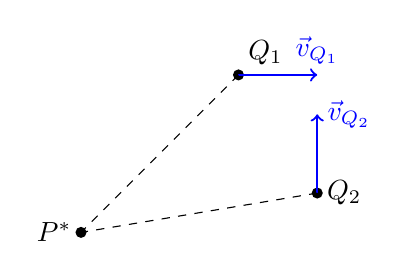
\begin{tikzpicture}
    % Costruzione grafica per P*
    \coordinate (P) at (0,0);
    \coordinate (Q1) at (2,2);
    \coordinate (Q2) at (3,0.5);
    
    \node[left] at (P) {$P^*$};
    \node[above right] at (Q1) {$Q_1$};
    \node[right] at (Q2) {$Q_2$};
    
    \fill (P) circle (2pt);
    \fill (Q1) circle (2pt);
    \fill (Q2) circle (2pt);
    
    % Velocità di Q1 (orizzontale)
    \draw[->,thick,blue] (Q1) -- ++(1,0) node[above] {$\vec{v}_{Q_1}$};
    % Perpendicolare da Q1
    \draw[dashed] (Q1) -- (P);
    
    % Velocità di Q2 (verticale)
    \draw[->,thick,blue] (Q2) -- ++(0,1) node[right] {$\vec{v}_{Q_2}$};
    % Perpendicolare da Q2
    \draw[dashed] (Q2) -- (P);
\end{tikzpicture}
